\documentclass[a4paper,12pt]{article} %размер бумаги устанавливаем А4, шрифт 12пунктов
% \usepackage[T2A]{fontenc}
\usepackage[utf8]{inputenc}%кодировка
\usepackage[english,russian]{babel}%используем русский и английский языки с переносами
% \usepackage{amssymb,amsfonts,amsmath,cite,enumerate,float,indentfirst} %пакеты расширений
\usepackage[pdftex]{graphicx} %вставка графики
\graphicspath{{images/}}%путь к рисункам
\usepackage{minted}
\usepackage{listings}

% \makeatletter
% \renewcommand{\@biblabel}[1]{#1.} % Заменяем библиографию с квадратных скобок на точку:
% \makeatother

\usepackage{geometry} % Меняем поля страницы
\geometry{left=2cm}% левое поле
\geometry{right=1.5cm}% правое поле
\geometry{top=1cm}% верхнее поле
\geometry{bottom=2cm}% нижнее поле

% \usepackage{hyperref}
% \hypersetup{%
%     pdfborder = {0 0 0}
% }
\usepackage[hidelinks]{hyperref}

\usepackage{wrapfig}

% \renewcommand{\theenumi}{\arabic{enumi}}% Меняем везде перечисления на цифра.цифра
% \renewcommand{\labelenumi}{\arabic{enumi}}% Меняем везде перечисления на цифра.цифра
% \renewcommand{\theenumii}{.\arabic{enumii}}% Меняем везде перечисления на цифра.цифра
% \renewcommand{\labelenumii}{\arabic{enumi}.\arabic{enumii}.}% Меняем везде перечисления на цифра.цифра
% \renewcommand{\theenumiii}{.\arabic{enumiii}}% Меняем везде перечисления на цифра.цифра
% \renewcommand{\labelenumiii}{\arabic{enumi}.\arabic{enumii}.\arabic{enumiii}.}% Меняем везде перечисления на цифра.цифра

% \newcommand{\imgh}[3]{\begin{figure}[h]\center{\includegraphics[width=#1]{#2}}\caption{#3}\label{ris:#2}\end{figure}}

\begin{document}
\begin{titlepage}
\newpage

\begin{center}
	\textbf{
		Санкт-Петербургский Государственный Университет \\
		Математико-механический факультет \\
	}
	Кафедра системного программирования
\end{center}

\vspace{15em}

\begin{center}
\Large Форматирование текста программ на основе комбинаторов, сопоставления с образцом и синтаксических шаблонов \\ 
\end{center}

\vspace{2em}

\begin{center}
Курсовая работа студента 445 группы \\
Подкопаева Антона Викторовича

% \textsc{\textbf{Название темы работы \linebreak длинное очень, набранное в \LaTeX{}}}
\end{center}

\vspace{10em}

Научный руководитель:\\
доцент кафедры системного программирования \dotfill
Д. Ю. Булычев

% \newbox{\lbox}
% \savebox{\lbox}{\hbox{Пупкин Иван Иванович}}
% \newlength{\maxl}
% \setlength{\maxl}{\wd\lbox}
% \hfill\parbox{11cm}{
% \hspace*{5cm}\hspace*{-5cm}Студент:\hfill\hbox to\maxl{Тест Пользователь\hfill}\\
% \hspace*{5cm}\hspace*{-5cm}Преподаватель:\hfill\hbox to\maxl{Пупкин Иван Иванович}\\
% \\
% \hspace*{5cm}\hspace*{-5cm}Группа:\hfill\hbox to\maxl{NNN}\\
% }


\vspace{\fill}

\begin{center}
Санкт-Петербург \\2013
\end{center}

\end{titlepage}
\newpage
\tableofcontents % это оглавление, которое генерируется автоматически
\newpage
\section*{Введение}
\addcontentsline{toc}{section}{Введение}

% На данный момент в программных системах самым распространенным представлением информации, которая создается пользователем или демонстрируется ему, является текстовое представление. Оно удобно по многим причинам, но у него есть существенный недостаток - часто без дополнительного стилизирования текстовая информация слишком тяжело воспринимается. При отображении данных для пользователя необходимо явственным образом сохранять изначальную структуру информации. В большинстве случаев такое стилизирование сводится к форматированию текста, то есть добавлению или удалению не несущих информацию символов, другому преобразованию текста без изменения его семантики. Данное преобразование называется \textbf{pretty printing}.

С появлением первых языков программирования особую важность приобрели языковые процессоры. \textbf{Языковой процессор} (\textbf{ЯП}) --- это программное средство, принимающее на вход программу в виде текста на некотором языке (программирования, разметки и т. д.) и решающее определенную задачу над этой программой. К языковым процессорам можно отнести: компиляторы, суперкомпиляторы, интерпретаторы, средства статического анализа кода, декомпиляторы, средства рефакторинга, средства реинжиниринга, интегрированные среды разработки (IDE) и др.

Первым этапом работы ЯП является \textbf{синтаксический анализ}, то есть сопоставление входного текста (линейной последовательности лексем) с формальной грамматикой языка. В результате работы синтаксического анализатора ЯП получает древовидное представление программы, над которым потом происходит основная работа.

Достаточно часто возникает задача показать пользователю промежуточный или конечный результат обработки кода.
Следовательно, необходимо вернуться к текстовому представлению программы, то есть провести процедуру, обратную синтаксическому анализу. Такая задача называется \textbf{pretty printing}, а соответствующий инструмент --- \textbf{pretty printer}. Далее этот инструмент мы будем называть \textbf{принтером}.

Одной из проблем, возникающей при разработке принтера, является то, что критерии качества его работы трудно формализуемы.
Очевидно, что одного соответствия с точки зрения синтаксиса и семантики полученного кода и древовидного представления недостаточно. Рассмотрим программы на рисунках~\ref{fig:wikiExUnfor} и \ref{fig:wikiExBSD}.

\begin{figure}[h!]
	\centering
	% \inputminted{c}{codes/wikiExUnfor.c}
	\lstinputlisting[language=C]{codes/wikiExUnfor.c}
	\caption{Неформатированный код}
	\label{fig:wikiExUnfor}
\end{figure}

\begin{figure}[h!]
	\centering
	% \inputminted{c}{codes/wikiExBSD.c}
	\lstinputlisting[language=C]{codes/wikiExBSD.c}
	\caption{Форматированный код}
	\label{fig:wikiExBSD}
\end{figure}

Они эквиваленты синтаксически и семантически с точки зрения компилятора C, но для пользователя вариант с рисунка~\ref{fig:wikiExBSD} предпочтительней, так как он проще для восприятия. Как мы видим, при отображении данных необходимо явным для пользователя образом сохранять иерархическую структуру информации. В большинстве случаев решение этой задачи сводится к добавлению или удалению символов, не несущих информации для синтаксического анализа, или другому преобразованию текста без изменения его семантики.

Кроме того определенную сложность в описание и исполнение конкретного принтера вносит тот факт, что в большинстве случаев нельзя однозначным образом сопоставить синтаксическую конструкцию с единственным представлением. Необходима вариативность в зависимости от дополнительных условий, наложенных на результат его работы.

Рассмотрим небольшой пример. Пользователь задает условие вида: “последовательные операторы пишутся на одной строке, если помещаются в N символов, а иначе --- на разных строках”.

\begin{figure}[h!]
	\centering
	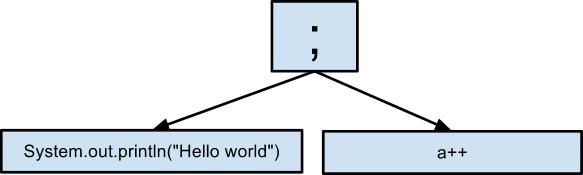
\includegraphics[width=0.8\textwidth]{seqTree}
	\caption{Последовательные операторы}
	\label{fig:seqImage}
\end{figure}

На рисунке~\ref{fig:seqImage} изображено синтаксическое дерево последовательности двух операторов. Такое дерево, согласно заданному правилу, может быть напечатано одним из двух вариантов (рисунки ~\ref{fig:seqCode1}, ~\ref{fig:seqCode2}).

\begin{figure}[h!]
	\centering
	% \inputminted{c}{codes/seqCode1.java}
	\lstinputlisting[language=Java]{codes/seqCode1.java}
	\caption{Последовательные операторы в строчку}
	\label{fig:seqCode1}
\end{figure}

\begin{figure}[h!]
	\centering
	% \inputminted{c}{codes/seqCode2.java}
	\lstinputlisting[language=Java]{codes/seqCode2.java}
	\caption{Последовательные операторы в несколько строк}
	\label{fig:seqCode2}
\end{figure}

Выбор происходит в зависимости от ширины вывода. Так, при ширине равной 35 символов (длина строки <<System.out.println(“Hello world”); >>), должен выбираться вариант, изображенный на рисунке~\ref{fig:seqCode2}, так как код на рисунке~\ref{fig:seqCode1} имеет ширину более 35 символов.
Могут быть заданы и более сложные условия.

Рассмотрим другой пример. Пусть нам нужно текстовое представление синтаксического дерева конструкции <<\lstinline{if}>>, и заданы шаблонами c рисунков~\ref{fig:ifTemplate2} и \ref{fig:ifTemplate1}, причем вариант, изображенный на рисунке~\ref{fig:ifTemplate2} выбирается в случае, если условие и ветки могут быть напечатаны в одну строчку.

\begin{figure}[h!]
	\begin{subfigure}[b]{0.45\textwidth}
		% \inputminted{haskell}{codes/ifTemplate2.hs}
		\lstinputlisting[language=Haskell]{codes/ifTemplate2.hs}
		\caption{}
		\label{fig:ifTemplate2}
	\end{subfigure}
	\hspace{1cm}
	\begin{subfigure}[b]{0.45\textwidth}
		% \inputminted{haskell}{codes/ifTemplate1.hs}
		\lstinputlisting[language=Haskell]{codes/ifTemplate1.hs}
		\caption{}
		\label{fig:ifTemplate1}
	\end{subfigure}
	\caption{Представления для конструкции <<\lstinline{if}>>}
\end{figure}


Тогда для деревьев, представленных на рисунках \ref{fig:ifImage1} и \ref{fig:ifImage2}, будут напечатаны коды с рисунков \ref{fig:ifCode1} и \ref{fig:ifCode2} соответственно.

\begin{figure}[h!]
	\begin{subfigure}[b]{0.60\linewidth}
		\centering
		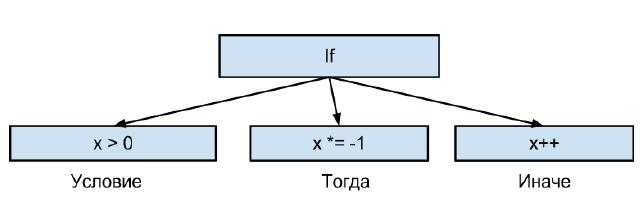
\includegraphics[width=\textwidth]{if1}
		\caption{}
		\label{fig:ifImage1}
	\end{subfigure}
	\hspace{0.5cm}
	\begin{subfigure}[b]{0.30\linewidth}
		\centering
		% \inputminted{haskell}{codes/ifCode1.hs}
		\lstinputlisting[language=Haskell]{codes/ifCode1.hs}
		\caption{}
		\label{fig:ifCode1}
	\end{subfigure}

	\caption{Использование представления с рис.~\ref{fig:ifTemplate2}}
\end{figure}

\begin{figure}[h!]
	\begin{subfigure}[b]{0.60\linewidth}
		\centering
		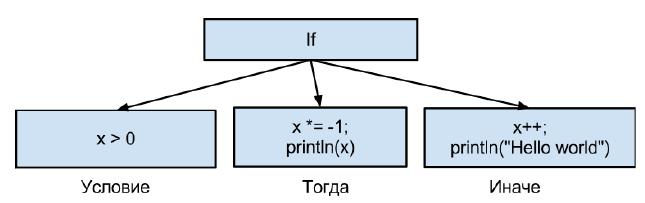
\includegraphics[width=\textwidth]{if2}
		\caption{}
		\label{fig:ifImage2}
	\end{subfigure}
	\hspace{0.5cm}
	\begin{subfigure}[b]{0.30\linewidth}
		\centering
		% \inputminted{haskell}{codes/ifCode2.hs}
		\lstinputlisting[language=Haskell]{codes/ifCode2.hs}
		\caption{}
		\label{fig:ifCode2}
	\end{subfigure}

	\caption{Использование представления с рис.~\ref{fig:ifTemplate1}}
\end{figure}

% Постановка задачи
То, что не существует четких критериев красоты кода, а также отсутствие библиотек, предоставляющих возможность описать принтер в виде, подобном
рассмотренному примеру с конструкцией <<\lstinline{if}>>, то есть с помощью шаблонов, часто приводит к тому, что принтеры становятся крайне сложными и наполненными эвристиками.

Задачей данной работы было изучение существующих подходов к построению принтеров в рамках функциональных языков программирования и разработка способа определения принтеров с помощью синтаксических шаблонов.
\newpage
\section{Обзор существующих библиотек}

В рамках исследования был проведен анализ существующих pretty printer библиотек на основе комбинаторов.
% возможно, рассказать о комбинаторах

\subsection{Библиотека Джона Хьюза}

Библиотека Джона Хьюза, описанная в \cite{hughes}, явялется первой комбинаторной pretty printing библиотекой. Она основана на алгоритме, предложенном Дереком Оппеном в \cite{oppen}, по сути является его реализацией в функциональном стиле на Haskell. Также библиотека Джона Хьюза, расширенная Саймоном Пейтоном Джонсом \cite{peytonJones}, является стандартной pretty print библиотекой для Haskell.

% рассказать об оптимальном

В данной библиотеке ключевым типом является \textbf{Doc}. Основные комбинаторы для составления документа:
\inputminted{haskell}{codes/hughesBasicOperators.hs}

Так с помощью функции \textbf{text} по строке получается документ, оператор \textbf{(<>)} соединяет два документа горизонтально (см. рисунок~\ref{fig:hughesHorComp}), а оператор \textbf{(\$\$)} соединяет документы вертикально (см. рисунок~\ref{fig:hughesVertComp}).

\begin{figure}[h!]
	\begin{minipage}[b]{0.45\linewidth}
		\centering
		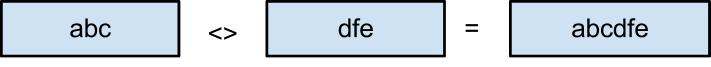
\includegraphics[width=\textwidth]{hughesHorComp}
		\caption{}
		\label{fig:hughesHorComp}
	\end{minipage}
	\hspace{0.5cm}
	\begin{minipage}[b]{0.45\linewidth}
		\centering
		
\includegraphics[width=\textwidth]{hughesVertComp}
		\caption{}
		\label{fig:hughesVertComp}
	\end{minipage}
\end{figure}

Элемент типа \textbf{Doc} может быть переведен в строку с помощью функции \textbf{pretty}.
\inputminted{haskell}{codes/hughesPretty.hs}
Кроме самого документа, функция \textbf{pretty} также принимает два числа: максимальную длину и максимальную наполненность строки. Здесь максимальная наполненность строки значит длину текста без выдущих пробельных символов.


\newpage
\newpage
\addcontentsline{toc}{section}{Список литературы}

% \bibliographystyle{plain}
% \bibliography{articles}

\begin{thebibliography}{9001}
  
	\bibitem{swierstra} Azero P., Swierstra S. D. Optimal Pretty-Printing Combinators // http://www.cs.ruu.nl/groups/ST/Software/PP/.

	\bibitem{hughes} Hughes J. The Design of a Pretty-printing Library // Advanced Functional Programming. Springer Verlag. 1995. P. 53-96.

	\bibitem{peytonJones} Peyton Jones S. Haskell Pretty-printer Library // 1997. http://www.haskell.org/ghc/docs/latest/html/libraries/pretty-1.1.1.0/Text-PrettyPrint.html.

	\bibitem{oppen} Oppen D. Pretty Printing // Stanford Verification Group. Report No. 13. Computer Science Department Report No. STAN-CS-79-770. 1979.

	\bibitem{wadler} Wadler P. A Prettier Printer // Journal of Functional Programming. Palgrave Macmillan. 1998. P.223-244.

\end{thebibliography}
%\input{RefProject-Description}% это описание
%\input{RefProject-Algoritm}% это описание алгоритмов
%\input{RefProject-Finish}% заключение
%\input{RefProject-App}% приложение
\end{document}
